% Options for packages loaded elsewhere
\PassOptionsToPackage{unicode}{hyperref}
\PassOptionsToPackage{hyphens}{url}
%
\documentclass[
]{article}
\usepackage{amsmath,amssymb}
\usepackage{lmodern}
\usepackage{iftex}
\ifPDFTeX
  \usepackage[T1]{fontenc}
  \usepackage[utf8]{inputenc}
  \usepackage{textcomp} % provide euro and other symbols
\else % if luatex or xetex
  \usepackage{unicode-math}
  \defaultfontfeatures{Scale=MatchLowercase}
  \defaultfontfeatures[\rmfamily]{Ligatures=TeX,Scale=1}
\fi
% Use upquote if available, for straight quotes in verbatim environments
\IfFileExists{upquote.sty}{\usepackage{upquote}}{}
\IfFileExists{microtype.sty}{% use microtype if available
  \usepackage[]{microtype}
  \UseMicrotypeSet[protrusion]{basicmath} % disable protrusion for tt fonts
}{}
\makeatletter
\@ifundefined{KOMAClassName}{% if non-KOMA class
  \IfFileExists{parskip.sty}{%
    \usepackage{parskip}
  }{% else
    \setlength{\parindent}{0pt}
    \setlength{\parskip}{6pt plus 2pt minus 1pt}}
}{% if KOMA class
  \KOMAoptions{parskip=half}}
\makeatother
\usepackage{xcolor}
\IfFileExists{xurl.sty}{\usepackage{xurl}}{} % add URL line breaks if available
\IfFileExists{bookmark.sty}{\usepackage{bookmark}}{\usepackage{hyperref}}
\hypersetup{
  pdftitle={Relatório trabalho prático 4},
  pdfauthor={César A. Galvão 19/0011572; Gabriela Carneiro 18/0120816},
  hidelinks,
  pdfcreator={LaTeX via pandoc}}
\urlstyle{same} % disable monospaced font for URLs
\usepackage[margin=1in]{geometry}
\usepackage{color}
\usepackage{fancyvrb}
\newcommand{\VerbBar}{|}
\newcommand{\VERB}{\Verb[commandchars=\\\{\}]}
\DefineVerbatimEnvironment{Highlighting}{Verbatim}{commandchars=\\\{\}}
% Add ',fontsize=\small' for more characters per line
\usepackage{framed}
\definecolor{shadecolor}{RGB}{248,248,248}
\newenvironment{Shaded}{\begin{snugshade}}{\end{snugshade}}
\newcommand{\AlertTok}[1]{\textcolor[rgb]{0.94,0.16,0.16}{#1}}
\newcommand{\AnnotationTok}[1]{\textcolor[rgb]{0.56,0.35,0.01}{\textbf{\textit{#1}}}}
\newcommand{\AttributeTok}[1]{\textcolor[rgb]{0.77,0.63,0.00}{#1}}
\newcommand{\BaseNTok}[1]{\textcolor[rgb]{0.00,0.00,0.81}{#1}}
\newcommand{\BuiltInTok}[1]{#1}
\newcommand{\CharTok}[1]{\textcolor[rgb]{0.31,0.60,0.02}{#1}}
\newcommand{\CommentTok}[1]{\textcolor[rgb]{0.56,0.35,0.01}{\textit{#1}}}
\newcommand{\CommentVarTok}[1]{\textcolor[rgb]{0.56,0.35,0.01}{\textbf{\textit{#1}}}}
\newcommand{\ConstantTok}[1]{\textcolor[rgb]{0.00,0.00,0.00}{#1}}
\newcommand{\ControlFlowTok}[1]{\textcolor[rgb]{0.13,0.29,0.53}{\textbf{#1}}}
\newcommand{\DataTypeTok}[1]{\textcolor[rgb]{0.13,0.29,0.53}{#1}}
\newcommand{\DecValTok}[1]{\textcolor[rgb]{0.00,0.00,0.81}{#1}}
\newcommand{\DocumentationTok}[1]{\textcolor[rgb]{0.56,0.35,0.01}{\textbf{\textit{#1}}}}
\newcommand{\ErrorTok}[1]{\textcolor[rgb]{0.64,0.00,0.00}{\textbf{#1}}}
\newcommand{\ExtensionTok}[1]{#1}
\newcommand{\FloatTok}[1]{\textcolor[rgb]{0.00,0.00,0.81}{#1}}
\newcommand{\FunctionTok}[1]{\textcolor[rgb]{0.00,0.00,0.00}{#1}}
\newcommand{\ImportTok}[1]{#1}
\newcommand{\InformationTok}[1]{\textcolor[rgb]{0.56,0.35,0.01}{\textbf{\textit{#1}}}}
\newcommand{\KeywordTok}[1]{\textcolor[rgb]{0.13,0.29,0.53}{\textbf{#1}}}
\newcommand{\NormalTok}[1]{#1}
\newcommand{\OperatorTok}[1]{\textcolor[rgb]{0.81,0.36,0.00}{\textbf{#1}}}
\newcommand{\OtherTok}[1]{\textcolor[rgb]{0.56,0.35,0.01}{#1}}
\newcommand{\PreprocessorTok}[1]{\textcolor[rgb]{0.56,0.35,0.01}{\textit{#1}}}
\newcommand{\RegionMarkerTok}[1]{#1}
\newcommand{\SpecialCharTok}[1]{\textcolor[rgb]{0.00,0.00,0.00}{#1}}
\newcommand{\SpecialStringTok}[1]{\textcolor[rgb]{0.31,0.60,0.02}{#1}}
\newcommand{\StringTok}[1]{\textcolor[rgb]{0.31,0.60,0.02}{#1}}
\newcommand{\VariableTok}[1]{\textcolor[rgb]{0.00,0.00,0.00}{#1}}
\newcommand{\VerbatimStringTok}[1]{\textcolor[rgb]{0.31,0.60,0.02}{#1}}
\newcommand{\WarningTok}[1]{\textcolor[rgb]{0.56,0.35,0.01}{\textbf{\textit{#1}}}}
\usepackage{graphicx}
\makeatletter
\def\maxwidth{\ifdim\Gin@nat@width>\linewidth\linewidth\else\Gin@nat@width\fi}
\def\maxheight{\ifdim\Gin@nat@height>\textheight\textheight\else\Gin@nat@height\fi}
\makeatother
% Scale images if necessary, so that they will not overflow the page
% margins by default, and it is still possible to overwrite the defaults
% using explicit options in \includegraphics[width, height, ...]{}
\setkeys{Gin}{width=\maxwidth,height=\maxheight,keepaspectratio}
% Set default figure placement to htbp
\makeatletter
\def\fps@figure{htbp}
\makeatother
\setlength{\emergencystretch}{3em} % prevent overfull lines
\providecommand{\tightlist}{%
  \setlength{\itemsep}{0pt}\setlength{\parskip}{0pt}}
\setcounter{secnumdepth}{5}
\usepackage{helvet} \renewcommand\familydefault{\sfdefault}
\usepackage{booktabs}
\usepackage{longtable}
\usepackage{array}
\usepackage{multirow}
\usepackage{wrapfig}
\usepackage{float}
\usepackage{colortbl}
\usepackage{pdflscape}
\usepackage{tabu}
\usepackage{threeparttable}
\usepackage{threeparttablex}
\usepackage[normalem]{ulem}
\usepackage{makecell}
\usepackage{xcolor}
\ifLuaTeX
  \usepackage{selnolig}  % disable illegal ligatures
\fi

\title{Relatório trabalho prático 4}
\author{César A. Galvão 19/0011572 \and Gabriela Carneiro 18/0120816}
\date{11 de September de 2022}

\begin{document}
\maketitle

\newpage{}

{
\setcounter{tocdepth}{2}
\tableofcontents
}
\let\oldsection\section
\renewcommand\section{\clearpage\oldsection}

\hypertarget{resumo}{%
\section{Resumo}\label{resumo}}

Nesta atividade foram implementadas em R um algoritmo EM e um método
MCMC. Para cada algoritmo, foram estimados três parâmetros:
probabilidade de o lote vir da máquina A \((p)\) e a probabilidade de
que, dado que uma determinada peça tenha sido produzida pela máquina A
ou B, a peça seja defeituosa \((\theta_A, \theta_B)\). Por fim, são
apresentados histogramas com a função de probabilidade conjunta obtida
pelos parâmetros estimados sobreposta em formato de pontos.\footnote{Todos
  os documentos desse relatório podem ser verificados no repositório
  \url{https://github.com/cesar-galvao/Estatistica-computacional}}

\hypertarget{muxe9todo}{%
\section{Método}\label{muxe9todo}}

\hypertarget{muxe9todo-em}{%
\subsection{Método EM}\label{muxe9todo-em}}

Na presença de variáveis ausentes ou outras condições semelhantes, EM
(Expectation-Maximization) é um algoritmo seguro que garante a
convergência para ao menos um máximo local. Cada iteração do algoritmo
EM consiste em duas etapas. Primeiramente, a etapa \emph{Expectation}
(E), consiste em atribuir uma distribuição de probabilidades para os
complementos dos dados, dado o modelo atual. Em seguida, os parâmetros
do modelo são reestimados (Etapa M). Este procedimento iterativo é
repetido até que algum critério de convergência seja satisfeito.

O algoritmo EM tem duas vantagens principais que o torna uma boa escolha
para solucionar problemas de máxima verossimilhança:

\begin{enumerate}
\def\labelenumi{\arabic{enumi}.}
\tightlist
\item
  O algoritmo EM fornece condição para satisfazer automatecamente
  restrições probabilísticas de \emph{mixture models}, que são modelos
  probabilísticos para representar a presença de subpopulações dentro de
  uma população maior, sem que seja necessário que haja um conjunto de
  dados observado para identificar a subpopulação à qual uma observação
  individual pertence. Outras abordagens de otimização exigem mais
  custos computacionais e o desenvolvimentos de algoritmos mais
  complexos.
\item
  O algoritmo EM garante um sequência crescente de verossimilhança e uma
  convergência monotônica segura.
\end{enumerate}

É importante ressaltar que a seleção de valores iniciais é um passo
muito importante para este procedimento iterativo, uma vez que a seleção
apropriada de valores iniciais pode aumentar a velocidade de
convergência. Mais importante ainda, a escolha dos valores iniciais
auxilia o algoritmo a evitar ótimos locais para alcançar uma solução
global.

\hypertarget{amostrador-de-gibbs}{%
\subsection{Amostrador de Gibbs}\label{amostrador-de-gibbs}}

O amostrador de Gibbs é um dos tipos de método de simulação de Monte
Carlo via cadeia de Markov.

A ideia por trás desses métodos é simples e geral. Para amostrar uma
determinada distribuição de probabilidade, referida como a distribuição
alvo, uma cadeia de Markov adequada é construída com a propriedade de
que sua distribuição limitante e invariante seja a própria distribuição
alvo. Dependendo das especificidades do problema, a cadeia de Markov
pode ser construída pelo algoritmo de Metropolis-Hastings (M-H), sendo o
método de amostragem de Gibbs um caso especial do método Metropolis, ou
misturas desses dois algoritmos. Uma vez que a cadeia de Markov tenha
sido construída, uma amostra da distribuição alvo pode ser obtida
simulando a cadeia de Markov um grande número de vezes e registrando
seus valores. Em muitas situações, método de simulação de Monte Carlo
via cadeia de Markov fornece a única maneira prática de obter amostras
de distribuições de probabilidade de dimensões superiores.

No algoritmo de amostragem de Gibbs os parâmetros são agrupados em \(p\)
blocos \((\psi_1, ..., \psi_p)\) e cada bloco é amostrado de acordo com
a distribuição condicional completa do bloco \(\psi_k\), definida como a
distribuição condicional sob \(\pi\) de \(\psi_k\) dado todos os outros
blocos \(\psi_{-k}\) e denotada como \(\pi(\psi_k|\psi_{-k})\). Em
paralelo com o algoritmo M-H de vários blocos, o valor mais atual dos
blocos restantes é usado para derivar a distribuição condicional
completa de cada bloco.

\hypertarget{resultados}{%
\section{Resultados}\label{resultados}}

Para o método EM, obteve-se a seguinte estimativa final para os
parâmetros ao final de 29 iterações, considerando o critério de parada
\(|\gamma_i^{(k+1)} - \gamma_i^{(k)}| < 10^{-9}\):

\begin{longtable}{ccc}
\toprule
$\theta_A$ & $\theta_B$ & $p$\\
\midrule
\endfirsthead
\multicolumn{3}{@{}l}{\textit{(continued)}}\\
\toprule
$\theta_A$ & $\theta_B$ & $p$\\
\midrule
\endhead

\endfoot
\bottomrule
\endlastfoot
\cellcolor{gray!15}{0.0517882} & \cellcolor{gray!15}{0.0905156} & \cellcolor{gray!15}{0.6908754}\\*
\end{longtable}

A função de distribuição conjunta, com os parâmetros obtidos pelo
algoritmo EM, é definida

\begin{align}
  P(y) = (1-p)P(y|\theta_A) + p P(y|\theta_B). \label{conjunta}
\end{align}

Além disso, obteve-se o seguinte histograma com a função de distribuição
conjunta, representada por pontos:

\begin{figure}

{\centering 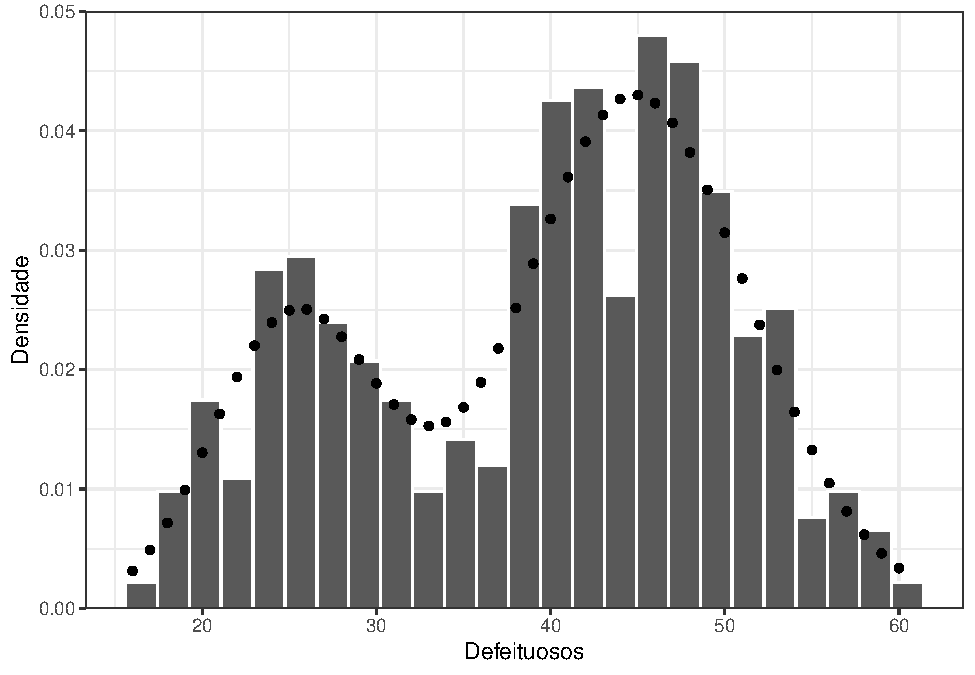
\includegraphics[width=0.6\linewidth]{relatorio_tp4_files/figure-latex/histograma-EM-1} 

}

\caption{Histograma de da amostra e função de distribuição conjunta com parâmetros obtidos pelo algoritmo EM.}\label{fig:histograma-EM}
\end{figure}

\newpage

Para o amostrador de Gibbs, as seguintes foram as estimativas para os
parâmetros:

\begin{longtable}{ccc}
\toprule
$\theta_A$ & $\theta_B$ & $p$\\
\midrule
\endfirsthead
\multicolumn{3}{@{}l}{\textit{(continued)}}\\
\toprule
$\theta_A$ & $\theta_B$ & $p$\\
\midrule
\endhead

\endfoot
\bottomrule
\endlastfoot
\cellcolor{gray!15}{0.0905063} & \cellcolor{gray!15}{0.0518119} & \cellcolor{gray!15}{0.3099991}\\*
\end{longtable}

Obteve-se o seguinte histograma com a mesma função de distribuição
conjunta (\ref{conjunta}), porém utilizando as novas estimativas,
representada por pontos:

\begin{figure}

{\centering 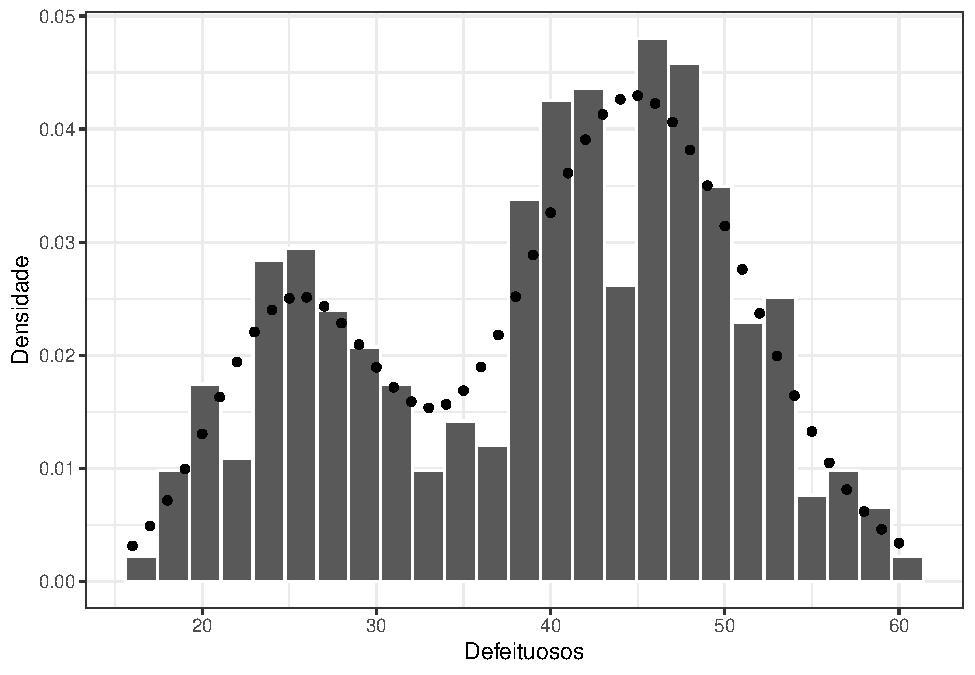
\includegraphics[width=0.6\linewidth]{relatorio_tp4_files/figure-latex/histograma-gibbs-1} 

}

\caption{Histograma de da amostra e função de distribuição conjunta com parâmetros obtidos pelo Amostrador de Gibbs.}\label{fig:histograma-gibbs}
\end{figure}

Finalmente, compara-se os métodos. Obtém-se uma diferença máxima de
0.00006 entre estimativas dos métodos, indicando pouca diferença no
cenário considerado -- duas subpopulações com medidas descritas por
variáveis binomiais.

O gráfico a seguir sugere uma certa homogeneidade das diferenças, o que
a princípio não sugeriria a preferência por um método específico para
esse conjunto de dados.

\begin{figure}

{\centering 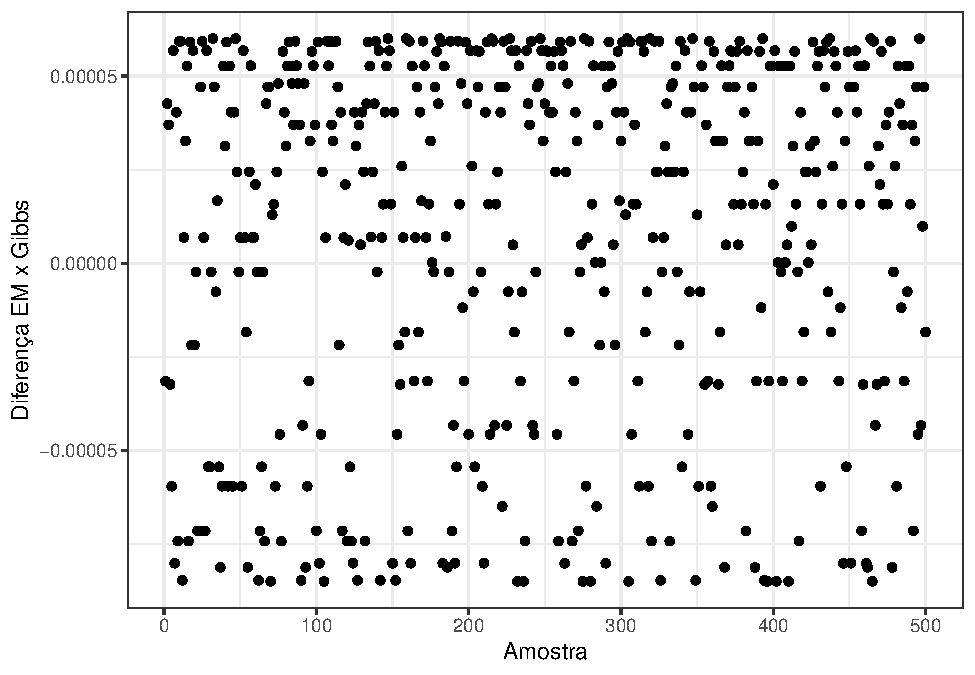
\includegraphics[width=0.6\linewidth]{relatorio_tp4_files/figure-latex/grafico-erros-1} 

}

\caption{Dispersão da diferença de estimação entre os métodos EM e Amostrador de Gibbs.}\label{fig:grafico-erros}
\end{figure}

\hypertarget{anexo-a---cuxf3digo-comentado}{%
\section*{Anexo A - código
comentado}\label{anexo-a---cuxf3digo-comentado}}
\addcontentsline{toc}{section}{Anexo A - código comentado}

\begin{Shaded}
\begin{Highlighting}[]
\CommentTok{\# entrada de dados {-}{-}{-}{-}}
\FunctionTok{library}\NormalTok{(tidyverse)}

\NormalTok{dados }\OtherTok{\textless{}{-}} \FunctionTok{read.csv2}\NormalTok{(}\StringTok{"data.csv"}\NormalTok{,}
                   \AttributeTok{col.names =} \FunctionTok{c}\NormalTok{(}\StringTok{"lote"}\NormalTok{, }\StringTok{"defeituosos"}\NormalTok{)) }\SpecialCharTok{\%\textgreater{}\%}
  \FunctionTok{mutate}\NormalTok{(}\AttributeTok{prop =}\NormalTok{ defeituosos}\SpecialCharTok{/}\DecValTok{500}\NormalTok{)}

\CommentTok{\# metodo EM {-}{-}{-}{-}}

\CommentTok{\#inicializando thetaA e thetaB}
\FunctionTok{set.seed}\NormalTok{(}\DecValTok{1234}\NormalTok{)}
\NormalTok{thetaA }\OtherTok{\textless{}{-}} \FunctionTok{sample}\NormalTok{(dados}\SpecialCharTok{$}\NormalTok{prop, }\DecValTok{1}\NormalTok{)}
\NormalTok{thetaB }\OtherTok{\textless{}{-}} \FunctionTok{sample}\NormalTok{(dados}\SpecialCharTok{$}\NormalTok{prop, }\DecValTok{1}\NormalTok{)}
\NormalTok{p }\OtherTok{\textless{}{-}} \FunctionTok{runif}\NormalTok{(}\DecValTok{1}\NormalTok{)}


\DocumentationTok{\#\# prepara dados de iteração com primeiro gamma {-}{-}{-}{-}}
\NormalTok{itera }\OtherTok{\textless{}{-}}\NormalTok{ dados }\SpecialCharTok{\%\textgreater{}\%} \CommentTok{\#gamma k+1}
  \FunctionTok{mutate}\NormalTok{(}\AttributeTok{gamma1 =}\NormalTok{ p}\SpecialCharTok{*}\FunctionTok{dbinom}\NormalTok{(defeituosos, }\AttributeTok{size =} \DecValTok{500}\NormalTok{, }\AttributeTok{prob =}\NormalTok{ thetaB)}\SpecialCharTok{/}
\NormalTok{           ((}\DecValTok{1}\SpecialCharTok{{-}}\NormalTok{p)}\SpecialCharTok{*}\FunctionTok{dbinom}\NormalTok{(defeituosos, }\AttributeTok{size =} \DecValTok{500}\NormalTok{, }\AttributeTok{prob =}\NormalTok{ thetaA)}\SpecialCharTok{+}
\NormalTok{              p}\SpecialCharTok{*}\FunctionTok{dbinom}\NormalTok{(defeituosos, }\AttributeTok{size =} \DecValTok{500}\NormalTok{, }\AttributeTok{prob =}\NormalTok{ thetaB)),}
         \AttributeTok{um\_menos\_gama1 =} \DecValTok{1}\SpecialCharTok{{-}}\NormalTok{gamma1)}

\NormalTok{itera}\SpecialCharTok{$}\NormalTok{dif }\OtherTok{\textless{}{-}} \DecValTok{1} \CommentTok{\#dif inicial para não travar o while}

\DocumentationTok{\#\# inicia iterações {-}{-}{-}{-}}

\NormalTok{contador }\OtherTok{\textless{}{-}} \DecValTok{0}

\ControlFlowTok{while}\NormalTok{(}\FunctionTok{any}\NormalTok{(itera}\SpecialCharTok{$}\NormalTok{dif }\SpecialCharTok{\textgreater{}} \DecValTok{10}\SpecialCharTok{\^{}}\NormalTok{(}\SpecialCharTok{{-}}\DecValTok{9}\NormalTok{)) }\SpecialCharTok{==} \ConstantTok{TRUE}\NormalTok{)\{}
  
\NormalTok{  contador }\OtherTok{\textless{}{-}}\NormalTok{ contador}\SpecialCharTok{+}\DecValTok{1}
  
\NormalTok{  itera}\SpecialCharTok{$}\NormalTok{gamma2 }\OtherTok{\textless{}{-}}\NormalTok{ itera}\SpecialCharTok{$}\NormalTok{gamma1 }\CommentTok{\#guarda o gama k}
  
  \DocumentationTok{\#\# M step {-}{-}{-}{-}}
  
\NormalTok{  thetaA }\OtherTok{\textless{}{-}} \FunctionTok{sum}\NormalTok{(itera}\SpecialCharTok{$}\NormalTok{defeituosos}\SpecialCharTok{*}\NormalTok{(itera}\SpecialCharTok{$}\NormalTok{um\_menos\_gama1))}\SpecialCharTok{/}\NormalTok{(}\DecValTok{500}\SpecialCharTok{*}\FunctionTok{sum}\NormalTok{(itera}\SpecialCharTok{$}\NormalTok{um\_menos\_gama1))}
\NormalTok{  thetaB }\OtherTok{\textless{}{-}} \FunctionTok{sum}\NormalTok{(itera}\SpecialCharTok{$}\NormalTok{defeituosos}\SpecialCharTok{*}\NormalTok{(itera}\SpecialCharTok{$}\NormalTok{gamma1))}\SpecialCharTok{/}\NormalTok{(}\DecValTok{500}\SpecialCharTok{*}\FunctionTok{sum}\NormalTok{(itera}\SpecialCharTok{$}\NormalTok{gamma1))}
\NormalTok{  p }\OtherTok{\textless{}{-}} \FunctionTok{sum}\NormalTok{(itera}\SpecialCharTok{$}\NormalTok{gamma1)}\SpecialCharTok{/}\DecValTok{500}
  
  \DocumentationTok{\#\# E step {-}{-}{-}{-}}
  
\NormalTok{  itera }\OtherTok{\textless{}{-}}\NormalTok{ itera }\SpecialCharTok{\%\textgreater{}\%}
    \FunctionTok{mutate}\NormalTok{(}\AttributeTok{gamma1 =}\NormalTok{ p}\SpecialCharTok{*}\FunctionTok{dbinom}\NormalTok{(defeituosos, }\AttributeTok{size =} \DecValTok{500}\NormalTok{, }\AttributeTok{prob =}\NormalTok{ thetaB)}\SpecialCharTok{/}
\NormalTok{             ((}\DecValTok{1}\SpecialCharTok{{-}}\NormalTok{p)}\SpecialCharTok{*}\FunctionTok{dbinom}\NormalTok{(defeituosos, }\AttributeTok{size =} \DecValTok{500}\NormalTok{, }\AttributeTok{prob =}\NormalTok{ thetaA)}\SpecialCharTok{+}
\NormalTok{                p}\SpecialCharTok{*}\FunctionTok{dbinom}\NormalTok{(defeituosos, }\AttributeTok{size =} \DecValTok{500}\NormalTok{, }\AttributeTok{prob =}\NormalTok{ thetaB)),}
           \AttributeTok{um\_menos\_gama1 =} \DecValTok{1}\SpecialCharTok{{-}}\NormalTok{gamma1)}
  
\NormalTok{  itera}\SpecialCharTok{$}\NormalTok{dif }\OtherTok{\textless{}{-}}\NormalTok{ itera}\SpecialCharTok{$}\NormalTok{gamma1 }\SpecialCharTok{{-}}\NormalTok{ itera}\SpecialCharTok{$}\NormalTok{gamma2}
\NormalTok{\}}

\DocumentationTok{\#\# funcao de probabilidade {-}{-}{-}{-}}
\NormalTok{Py }\OtherTok{\textless{}{-}} \ControlFlowTok{function}\NormalTok{(y)\{}
  \FunctionTok{return}\NormalTok{((}\DecValTok{1}\SpecialCharTok{{-}}\NormalTok{p)}\SpecialCharTok{*}\FunctionTok{dbinom}\NormalTok{(y, }\AttributeTok{size =} \DecValTok{500}\NormalTok{, }\AttributeTok{prob =}\NormalTok{ thetaA)}\SpecialCharTok{+}\NormalTok{ p}\SpecialCharTok{*}\FunctionTok{dbinom}\NormalTok{(y, }\AttributeTok{size =} \DecValTok{500}\NormalTok{, }\AttributeTok{prob =}\NormalTok{ thetaB))}
\NormalTok{\}}

\DocumentationTok{\#\# histograma {-}{-}{-}{-}}

\NormalTok{dados\_plot }\OtherTok{\textless{}{-}} \FunctionTok{data.frame}\NormalTok{(}\AttributeTok{x =}\NormalTok{ dados}\SpecialCharTok{$}\NormalTok{defeituosos, }\AttributeTok{y =} \FunctionTok{Py}\NormalTok{(dados}\SpecialCharTok{$}\NormalTok{defeituosos))}

\NormalTok{histograma\_em }\OtherTok{\textless{}{-}} \FunctionTok{ggplot}\NormalTok{(dados, }\FunctionTok{aes}\NormalTok{(}\AttributeTok{x =}\NormalTok{ defeituosos))}\SpecialCharTok{+}
  \FunctionTok{geom\_histogram}\NormalTok{(}\FunctionTok{aes}\NormalTok{(}\AttributeTok{y =}\NormalTok{ ..density..),}\AttributeTok{bins =} \DecValTok{25}\NormalTok{, }\AttributeTok{color =} \StringTok{"white"}\NormalTok{)}\SpecialCharTok{+}
  \FunctionTok{geom\_point}\NormalTok{(}\AttributeTok{data =}\NormalTok{ dados\_plot, }\FunctionTok{aes}\NormalTok{(}\AttributeTok{x =}\NormalTok{ x, }\AttributeTok{y =}\NormalTok{ y))}\SpecialCharTok{+}
  \FunctionTok{labs}\NormalTok{(}\AttributeTok{y =} \StringTok{"Densidade"}\NormalTok{, }\AttributeTok{x =} \StringTok{"Defeituosos"}\NormalTok{)}\SpecialCharTok{+}
  \FunctionTok{scale\_y\_continuous}\NormalTok{(}\AttributeTok{expand =} \FunctionTok{c}\NormalTok{(}\DecValTok{0}\NormalTok{,}\DecValTok{0}\NormalTok{), }\AttributeTok{limits =} \FunctionTok{c}\NormalTok{(}\DecValTok{0}\NormalTok{, }\FloatTok{0.05}\NormalTok{))}\SpecialCharTok{+}
  \FunctionTok{theme\_bw}\NormalTok{()}\SpecialCharTok{+}
  \FunctionTok{theme}\NormalTok{(}\CommentTok{\#panel.grid = element\_blank()\#,}
        \CommentTok{\# panel.border = element\_blank(),}
        \CommentTok{\# axis.line = element\_line()}
\NormalTok{        )}


\CommentTok{\# Amostrador de Gibbs {-}{-}{-}{-}}

\DocumentationTok{\#\# inicializando os parametros {-}{-}{-}{-}}

\NormalTok{thetaa }\OtherTok{\textless{}{-}} \FunctionTok{rbeta}\NormalTok{(}\DecValTok{1}\NormalTok{,}\DecValTok{1}\NormalTok{,}\DecValTok{1}\NormalTok{)}
\NormalTok{thetab }\OtherTok{\textless{}{-}} \FunctionTok{rbeta}\NormalTok{(}\DecValTok{1}\NormalTok{,}\DecValTok{1}\NormalTok{,}\DecValTok{1}\NormalTok{)}
\NormalTok{p2 }\OtherTok{\textless{}{-}} \FunctionTok{rbeta}\NormalTok{(}\DecValTok{1}\NormalTok{,}\DecValTok{1}\NormalTok{,}\DecValTok{1}\NormalTok{)}

\DocumentationTok{\#\# iterações {-}{-}{-}{-}}

\DocumentationTok{\#\#\# prepara dados de iteração com primeiro delta {-}{-}{-}{-}}
\NormalTok{itera2 }\OtherTok{\textless{}{-}}\NormalTok{ dados }\SpecialCharTok{\%\textgreater{}\%} 
  \FunctionTok{mutate}\NormalTok{(}\AttributeTok{delta1 =}\NormalTok{ (p2}\SpecialCharTok{*}\FunctionTok{dbinom}\NormalTok{(defeituosos, }\AttributeTok{size =} \DecValTok{500}\NormalTok{, }\AttributeTok{prob =}\NormalTok{ thetab))}\SpecialCharTok{/}
\NormalTok{           ((}\DecValTok{1}\SpecialCharTok{{-}}\NormalTok{p2)}\SpecialCharTok{*}\FunctionTok{dbinom}\NormalTok{(defeituosos, }\AttributeTok{size =} \DecValTok{500}\NormalTok{, }\AttributeTok{prob =}\NormalTok{ thetaa)}\SpecialCharTok{+}
\NormalTok{              p2}\SpecialCharTok{*}\FunctionTok{dbinom}\NormalTok{(defeituosos, }\AttributeTok{size =} \DecValTok{500}\NormalTok{, }\AttributeTok{prob =}\NormalTok{ thetab)),}
         \AttributeTok{um\_menos\_delta1 =} \DecValTok{1}\SpecialCharTok{{-}}\NormalTok{delta1)}
  
  
\DocumentationTok{\#\#\# inicia iterações {-}{-}{-}{-}}

\NormalTok{vec\_thetaa }\OtherTok{\textless{}{-}} \FunctionTok{c}\NormalTok{()}
\NormalTok{vec\_thetab }\OtherTok{\textless{}{-}} \FunctionTok{c}\NormalTok{()}
\NormalTok{vec\_p }\OtherTok{\textless{}{-}} \FunctionTok{c}\NormalTok{()}

\ControlFlowTok{for}\NormalTok{(i }\ControlFlowTok{in} \DecValTok{1}\SpecialCharTok{:}\DecValTok{20000}\NormalTok{)\{}
  \DocumentationTok{\#\#\#\# atualiza parametros {-}{-}{-}{-}}
  
\NormalTok{  alfaa }\OtherTok{\textless{}{-}} \DecValTok{1}\SpecialCharTok{+}\FunctionTok{sum}\NormalTok{(itera2}\SpecialCharTok{$}\NormalTok{defeituosos}\SpecialCharTok{*}\NormalTok{itera2}\SpecialCharTok{$}\NormalTok{um\_menos\_delta1)}
\NormalTok{  betaa }\OtherTok{\textless{}{-}} \DecValTok{1}\SpecialCharTok{+}\FunctionTok{sum}\NormalTok{((}\DecValTok{500}\SpecialCharTok{{-}}\NormalTok{itera2}\SpecialCharTok{$}\NormalTok{defeituosos)}\SpecialCharTok{*}\NormalTok{itera2}\SpecialCharTok{$}\NormalTok{um\_menos\_delta1)}
  
\NormalTok{  alfab }\OtherTok{\textless{}{-}} \DecValTok{1}\SpecialCharTok{+}\FunctionTok{sum}\NormalTok{(itera2}\SpecialCharTok{$}\NormalTok{defeituosos}\SpecialCharTok{*}\NormalTok{itera2}\SpecialCharTok{$}\NormalTok{delta1)}
\NormalTok{  betab }\OtherTok{\textless{}{-}} \DecValTok{1}\SpecialCharTok{+}\FunctionTok{sum}\NormalTok{((}\DecValTok{500}\SpecialCharTok{{-}}\NormalTok{itera2}\SpecialCharTok{$}\NormalTok{defeituosos)}\SpecialCharTok{*}\NormalTok{itera2}\SpecialCharTok{$}\NormalTok{delta1)}
  
\NormalTok{  alfap }\OtherTok{\textless{}{-}} \DecValTok{1}\SpecialCharTok{+}\FunctionTok{sum}\NormalTok{(itera2}\SpecialCharTok{$}\NormalTok{delta1)}
\NormalTok{  betap }\OtherTok{\textless{}{-}} \DecValTok{1}\SpecialCharTok{+}\FunctionTok{sum}\NormalTok{(itera2}\SpecialCharTok{$}\NormalTok{um\_menos\_delta1)}

\NormalTok{  thetaa }\OtherTok{\textless{}{-}} \FunctionTok{rbeta}\NormalTok{(}\DecValTok{1}\NormalTok{, alfaa, betaa)}
\NormalTok{  thetab }\OtherTok{\textless{}{-}} \FunctionTok{rbeta}\NormalTok{(}\DecValTok{1}\NormalTok{, alfab, betab)}
\NormalTok{  p2 }\OtherTok{\textless{}{-}} \FunctionTok{rbeta}\NormalTok{(}\DecValTok{1}\NormalTok{, alfap, betap)}
  
\NormalTok{  vec\_thetaa[i] }\OtherTok{\textless{}{-}}\NormalTok{ thetaa}
\NormalTok{  vec\_thetab[i] }\OtherTok{\textless{}{-}}\NormalTok{ thetab}
\NormalTok{  vec\_p[i] }\OtherTok{\textless{}{-}}\NormalTok{ p2}
  
  
  \DocumentationTok{\#\#\#\# atualiza delta {-}{-}{-}{-}}
  
\NormalTok{  itera2 }\OtherTok{\textless{}{-}}\NormalTok{ itera2 }\SpecialCharTok{\%\textgreater{}\%}
    \FunctionTok{mutate}\NormalTok{(}\AttributeTok{delta1 =}\NormalTok{ p2}\SpecialCharTok{*}\FunctionTok{dbinom}\NormalTok{(defeituosos, }\AttributeTok{size =} \DecValTok{500}\NormalTok{, }\AttributeTok{prob =}\NormalTok{ thetab)}\SpecialCharTok{/}
\NormalTok{             ((}\DecValTok{1}\SpecialCharTok{{-}}\NormalTok{p2)}\SpecialCharTok{*}\FunctionTok{dbinom}\NormalTok{(defeituosos, }\AttributeTok{size =} \DecValTok{500}\NormalTok{, }\AttributeTok{prob =}\NormalTok{ thetaa)}\SpecialCharTok{+}
\NormalTok{                p2}\SpecialCharTok{*}\FunctionTok{dbinom}\NormalTok{(defeituosos, }\AttributeTok{size =} \DecValTok{500}\NormalTok{, }\AttributeTok{prob =}\NormalTok{ thetab)),}
           \AttributeTok{um\_menos\_delta1 =} \DecValTok{1}\SpecialCharTok{{-}}\NormalTok{delta1)}
\NormalTok{\}}

\DocumentationTok{\#\# media das S ultimas amostras {-}{-}{-}{-}}

\NormalTok{thetaa\_final }\OtherTok{\textless{}{-}} \FunctionTok{mean}\NormalTok{(vec\_thetaa[}\DecValTok{10001}\SpecialCharTok{:}\DecValTok{20000}\NormalTok{])}
\NormalTok{thetab\_final }\OtherTok{\textless{}{-}} \FunctionTok{mean}\NormalTok{(vec\_thetab[}\DecValTok{10001}\SpecialCharTok{:}\DecValTok{20000}\NormalTok{])}
\NormalTok{p2\_final }\OtherTok{\textless{}{-}} \FunctionTok{mean}\NormalTok{(vec\_p[}\DecValTok{10001}\SpecialCharTok{:}\DecValTok{20000}\NormalTok{])}

\DocumentationTok{\#\# funcao de probabilidade {-}{-}{-}{-}}
\NormalTok{Py2 }\OtherTok{\textless{}{-}} \ControlFlowTok{function}\NormalTok{(y)\{}
  \FunctionTok{return}\NormalTok{((}\DecValTok{1}\SpecialCharTok{{-}}\NormalTok{p2\_final)}\SpecialCharTok{*}\FunctionTok{dbinom}\NormalTok{(y, }\AttributeTok{size =} \DecValTok{500}\NormalTok{, }\AttributeTok{prob =}\NormalTok{ thetaa\_final)}\SpecialCharTok{+}
\NormalTok{           p2\_final}\SpecialCharTok{*}\FunctionTok{dbinom}\NormalTok{(y, }\AttributeTok{size =} \DecValTok{500}\NormalTok{, }\AttributeTok{prob =}\NormalTok{ thetab\_final))}
\NormalTok{\}}

\DocumentationTok{\#\# histograma {-}{-}{-}{-}}

\NormalTok{dados\_plot2 }\OtherTok{\textless{}{-}} \FunctionTok{data.frame}\NormalTok{(}\AttributeTok{x =}\NormalTok{ dados}\SpecialCharTok{$}\NormalTok{defeituosos, }\AttributeTok{y =} \FunctionTok{Py2}\NormalTok{(dados}\SpecialCharTok{$}\NormalTok{defeituosos))}

\NormalTok{histograma\_gibbs }\OtherTok{\textless{}{-}} \FunctionTok{ggplot}\NormalTok{(dados, }\FunctionTok{aes}\NormalTok{(}\AttributeTok{x =}\NormalTok{ defeituosos))}\SpecialCharTok{+}
  \FunctionTok{geom\_histogram}\NormalTok{(}\FunctionTok{aes}\NormalTok{(}\AttributeTok{y =}\NormalTok{ ..density..),}\AttributeTok{bins =} \DecValTok{25}\NormalTok{, }\AttributeTok{color =} \StringTok{"white"}\NormalTok{)}\SpecialCharTok{+}
  \FunctionTok{geom\_point}\NormalTok{(}\AttributeTok{data =}\NormalTok{ dados\_plot2, }\FunctionTok{aes}\NormalTok{(}\AttributeTok{x =}\NormalTok{ x, }\AttributeTok{y =}\NormalTok{ y))}\SpecialCharTok{+}
  \FunctionTok{labs}\NormalTok{(}\AttributeTok{y =} \StringTok{"Densidade"}\NormalTok{, }\AttributeTok{x =} \StringTok{"Defeituosos"}\NormalTok{)}\SpecialCharTok{+}
  \CommentTok{\#scale\_y\_continuous(expand = c(0,0), limits = c(0, 0.05))+}
  \FunctionTok{theme\_bw}\NormalTok{()}\SpecialCharTok{+}
  \FunctionTok{theme}\NormalTok{(}\CommentTok{\#panel.grid = element\_blank()\#,}
    \CommentTok{\# panel.border = element\_blank(),}
    \CommentTok{\# axis.line = element\_line()}
\NormalTok{  )}

\CommentTok{\# diferença entre os métodos {-}{-}{-}{-}}

\NormalTok{diferencas }\OtherTok{\textless{}{-}} \FunctionTok{data.frame}\NormalTok{(}
  \AttributeTok{x =} \DecValTok{1}\SpecialCharTok{:}\DecValTok{500}\NormalTok{,}
  \AttributeTok{amostra =}\NormalTok{ dados}\SpecialCharTok{$}\NormalTok{defeituosos,}
  \AttributeTok{em =} \FunctionTok{Py}\NormalTok{(dados}\SpecialCharTok{$}\NormalTok{defeituosos),}
  \AttributeTok{gibbs =} \FunctionTok{Py2}\NormalTok{(dados}\SpecialCharTok{$}\NormalTok{defeituosos)}
\NormalTok{) }\SpecialCharTok{\%\textgreater{}\%} \FunctionTok{mutate}\NormalTok{(}\AttributeTok{diff =}\NormalTok{ em}\SpecialCharTok{{-}}\NormalTok{gibbs)}

\FunctionTok{options}\NormalTok{(}\AttributeTok{scipen =} \DecValTok{99999}\NormalTok{)}
\NormalTok{maxdiff }\OtherTok{\textless{}{-}} \FunctionTok{max}\NormalTok{(diferencas}\SpecialCharTok{$}\NormalTok{diff) }\SpecialCharTok{\%\textgreater{}\%} \FunctionTok{round}\NormalTok{(}\DecValTok{5}\NormalTok{)}

\NormalTok{graf\_diff }\OtherTok{\textless{}{-}} \FunctionTok{ggplot}\NormalTok{(diferencas, }\FunctionTok{aes}\NormalTok{(}\AttributeTok{x =}\NormalTok{ x, }\AttributeTok{y =}\NormalTok{ diff))}\SpecialCharTok{+}
  \FunctionTok{geom\_point}\NormalTok{()}\SpecialCharTok{+}
  \FunctionTok{labs}\NormalTok{(}\AttributeTok{y =} \StringTok{"Diferença EM x Gibbs"}\NormalTok{, }\AttributeTok{x =} \StringTok{"Amostra"}\NormalTok{)}\SpecialCharTok{+}
  \FunctionTok{theme\_bw}\NormalTok{()}
\end{Highlighting}
\end{Shaded}


\end{document}
